\documentclass[12pt,twoside]{scrreprt}
\usepackage[T1]{fontenc}
\usepackage{fancyvrb}
\usepackage[utf8]{inputenc}
\usepackage{lmodern}
\usepackage{textcomp}
\usepackage[francais]{babel, varioref}
\usepackage{graphicx}
\usepackage{listings}
\usepackage{float}
\usepackage{xspace}
\usepackage{amsmath}
\usepackage{amssymb}
\usepackage{calc}
\usepackage{listingsutf8}
\usepackage{color}
\usepackage{xcolor}
\usepackage{afterpage}
\usepackage[style=verbose-note,backend=bibtex]{biblatex}
\usepackage{url}
\usepackage[top=2.1cm,bottom=2.2cm,left=2cm,right=2cm]{geometry}
\usepackage[final]{pdfpages}
\usepackage{verbatim}
\usepackage{rotating, graphicx}
\usepackage{listings}

%Pour afficher le code c#	
\lstdefinestyle{sharpc}{language=[Sharp]C, frame=lr, rulecolor=\color{blue!80!black}}

% Pour sommaire cliquable 
\usepackage{hyperref} % Créer des liens et des signets
\hypersetup{
colorlinks=true, %colorise les liens
breaklinks=true, %permet le retour à la ligne dans les liens trop longs
urlcolor= blue, %couleur des hyperliens
linkcolor= black, %couleur des liens internes
citecolor=black,  %couleur des références
}

% Fichier de bibliographie
\bibliography{parties/biblio}

\usepackage{templateINSA}
\initINSA

% Tirte centre
\renewcommand\infoBig{PAO}
\renewcommand\infoSmall{Projet d'Approfondissement et d'Ouverture}

% Titre bas 
\title{Application d'aide pour les touristes étrangers}
\renewcommand\soustitre{}

% Auteurs
\author{ 
	\textbf{Étudiant:} Florian \bsc{Leriche} \\
	\textbf{Année:} 2016-2017\\
	\textbf{Lieu:} Rouen, France\\
	}

\begin{document}

% titleINSA : Page de garde 
% #1 : descendre le titre du milieu (en mm)
% #2 : lien de l'image de fond
% #3 : décalage sur X de l'image de fond (en mm)
% #4 : décalage sur Y de l'image de fond (en mm)
% #5 : largeur de l'image de fond de #5 (en mm)
% #6 : Crédit de l'image de fond
 \titleINSA{0}{img/eiffel.jpg}{0}{130}{220}{}
 

%Introduction
%\input{parties/00-Introduction.tex}
%\addcontentsline{toc}{chapter}{Introduction}

% Sommaire
\tableofcontents

% Parties
\chapter{Introduction}
Dans le cadre de ce projet d'approfondissement et d'ouverture nous allons concevoir une application Android permettant de fournir des informations ainsi que des conduites à tenir pour assister les touristes et les résidents étrangers en France. Les informations contenues au sein de cette dernière devront pouvoir transiter en format numérique aussi bien sur SmartPhone que sur tablette. L'application sera proposée à des utilisateurs de différentes nationalités dont le niveau de connaissances informatiques est très hétérogène c'est pourquoi elle devra être graphique, lisible et simple d'utilisation. \\
	Elle proposera tout ou partie des fonctionnalités suivantes :
\begin{itemize}
	\item Fournir les informations appropriées en fonction de la situation du touriste.
	\item Déclencher les conduites à tenir en cas d'urgence (appels téléphoniques vers différents services).
	\item Être multilingue.
	\item Supporter l'ajout de nouvelles fiches d'informations fournies par la gendarmerie ou langues.
	\item Avoir un module de géolocalisation permettant de guider le touriste vers l'adresse désignée (ambassade, consulat, police, gendarmerie ...).
\end{itemize}


\chapter{Spécifications}
\paragraph{}
	Dans cette partie, nous allons décrire en détail les différentes spécifications propres à notre projet. En premier lieu, nous commencerons par détailler les spécifications fonctionnelles en rappelant les diverses fonctionnalités attendues ainsi que nos objectifs. Nous appuierons nos explications à l'aide de maquette d'une étude des cas d'utilisation. En second lieu, nous présenterons les spécifications techniques de notre projet.

\section{Spécifications fonctionnelles}
\subsection{Présentation de la problématique}

	\paragraph{}
		Le but de ce projet d'approfondissement et d'ouverture est de concevoir une application Android permettant de fournir des informations ainsi que des conduites à tenir pour assister les touristes et les résidents étrangers en France. Les informations contenues au sein de cette dernière devront pouvoir transiter en format numérique aussi bien sur SmartPhone que sur tablette. L'application sera proposée à des utilisateurs de différentes nationalités dont le niveau de connaissances informatiques est très hétérogène c'est pourquoi elle devra être graphique, lisible et simple d'utilisation.
\subsection{Objectifs}
	
	\paragraph{}
		Nous allons maintenant présenter les différents objectifs que notre application devra atteindre. Ces derniers sont les suivants :
\begin{itemize}
	\item Fournir les informations appropriées en fonction de la situation du touriste.
	\item Déclencher les conduites à tenir en cas d'urgence (appels téléphoniques vers différents services).
	\item Être multilingue.
	\item Supporter l'ajout de nouvelles fiches d'informations fournies par la gendarmerie ou langues.
	\item Avoir un module de géolocalisation permettant de guider le touriste vers l'adresse désignée (ambassade, consulat, police, gendarmerie ...).
	\item Être graphique et très simple/rapide d'utilisation.
\end{itemize}
\subsection{Fonctionnalités}

\paragraph{}
	Nous allons maintenant détailler les différentes fonctionnalités qui feront parties intégrantes de notre projet.
	
\subsubsection{Conseils de prévention}
	\paragraph{}
		L'application devra permettre de fournir à l'utilisateur des informations appropriées en fonction de sa situation.Par exemple, elles peuvent concerner les transports en commun, les lieux publics, les hôtels ou encore les urgences. Ces informations auront pour objectif de conseiller un touriste étranger en France sur la conduite à adopter et la manière d'appréhender les choses lorsque celui-ci se trouve dans une situation particulière. Ces conseils sont fournis sous forme de fiche au format odt par la gendarmerie. De plus, celle-ci souhaite pouvoir ajouter de nouvelles informations lorsqu'elle le désire. Cependant, les connaissances informatique du client étant limitées, l'application devra permettre un ajout simplifié de ces informations. Par exemple par simple dépôt d'une fiche au bon format dans un dossier. Les situations seront symbolisées sous forme de liste de pictogrammes explicites auxquels seront adjoints des mots clés.

\subsubsection{Contacts}
	\paragraph{}
			L'application devra donner la possibilité à l'utilisateur d'accéder à une liste de contacts à appeler en cas d'urgence. Cette liste contiendra des numéros tels que ceux de la gendarmerie/police, des urgences, des pompiers ... Cette liste permettra de rediriger l'utilisateur sur son composeur téléphonique avec le numéro correspondant au contact qu'il souhaite appeler. Ainsi, celui-ci aura toujours le choix de confirmer ou d'annuler l'appel.
			
\subsubsection{Géolocalisation}
	\paragraph{}
			L'application devra contenir un module de géolocalisation et de navigation permettant de guider l'utilisateur vers la destination de son choix. Elle proposera une liste de destinations pouvant être utiles en fonction de la situation du touriste comme la gendarmerie, le consulat ou l'hôpital. Cette fonctionnalité aura pour objectif de renvoyer l'utilisateur sur Google Maps avec une recherche pré-effectuée pointant sur la direction qu'il aura choisi.
			
\subsubsection{Profil}
	\paragraph{}
			L'application devra permettre à l'utilisateur de pouvoir écrire ses informations personnelles ainsi que que les remarques médicales le concernant. Ces informations pourront être utilisées en cas d'urgence ou pour lister les différents problèmes concernant l'utilisateur.
			
\subsubsection{Multilingue}
	\paragraph{}
			L'application étant proposée à des touristes ou résidents étranger en France, celle-ci devra être multilingue. Les différents menus, listes de contacts et destinations seront donc traduits dans différentes langues. Les fiches de conseils devront également être traduites dans différentes langues. Elle devra proposer à l'utilisateur de choisir sa nationalité lors de sa première utilisation de l'application. De plus, elle devra également lui permettre de pouvoir modifier son choix et donc de changer de langue à tout moment.
			
			
\subsection{Cas d'utilisation}

Le diagramme présent sur la figure \ref{casUtilisations} permet de représenter les différents cas d'utilisation de l'application.
	
\begin{figure}[!h]
	\begin{center}
	
		\includegraphics[scale=0.6]{img/casUtilisations.png}
	    \caption{Diagramme de Cas d'Utilisation}
	    \label{casUtilisations} 
	
	\end{center}
\end{figure}

\newpage
\subsection{Maquette}

Les images \ref{maquette1} et \ref{maquette2} représentent la maquette permettant de décrire le cahier des charges et les spécifications d'interface qui ont été fourni pour la réalisation de l'application.

\begin{figure}[!h]
	\begin{center}
		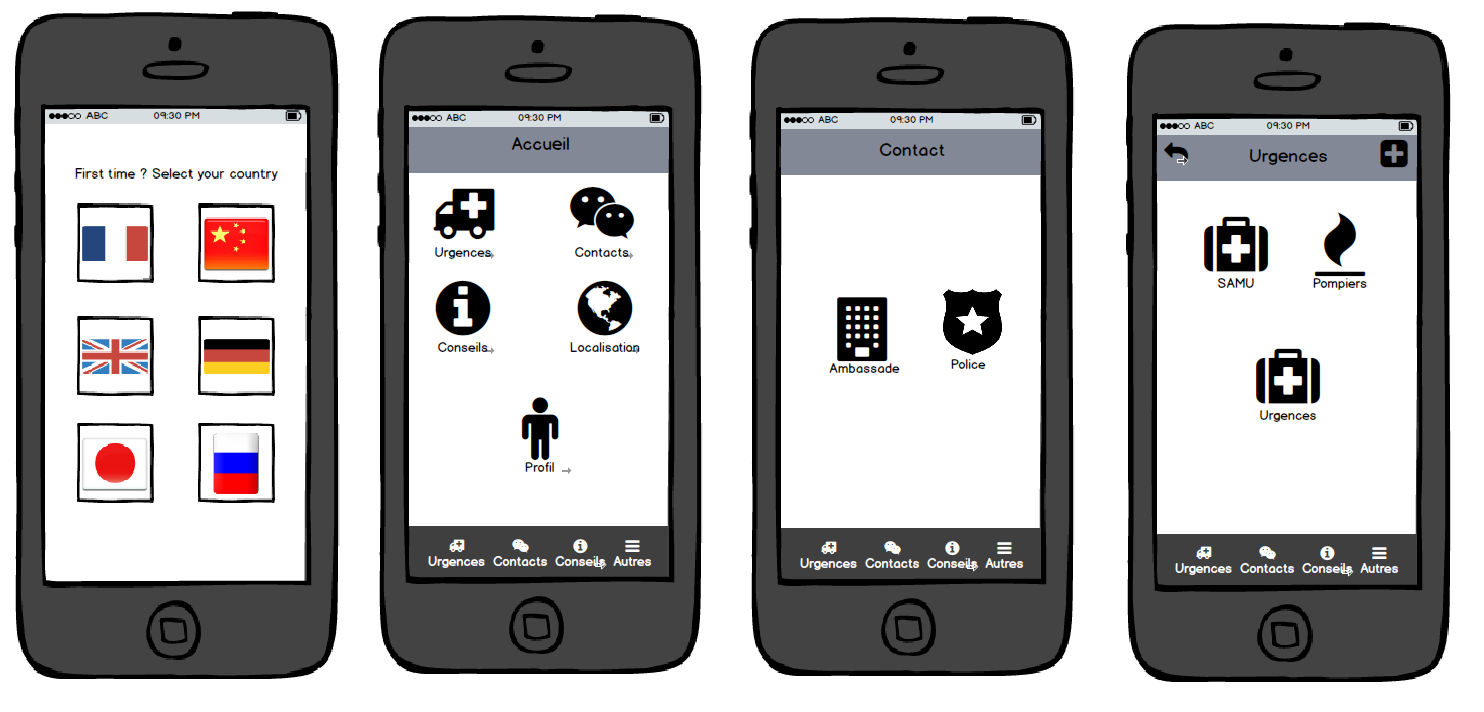
\includegraphics[scale=0.45]{img/maquette1.png}
		\caption{Maquette de l'application}
		\label{maquette1} 
	\end{center}
\end{figure}

\begin{figure}[!h]
	\begin{center}
		
		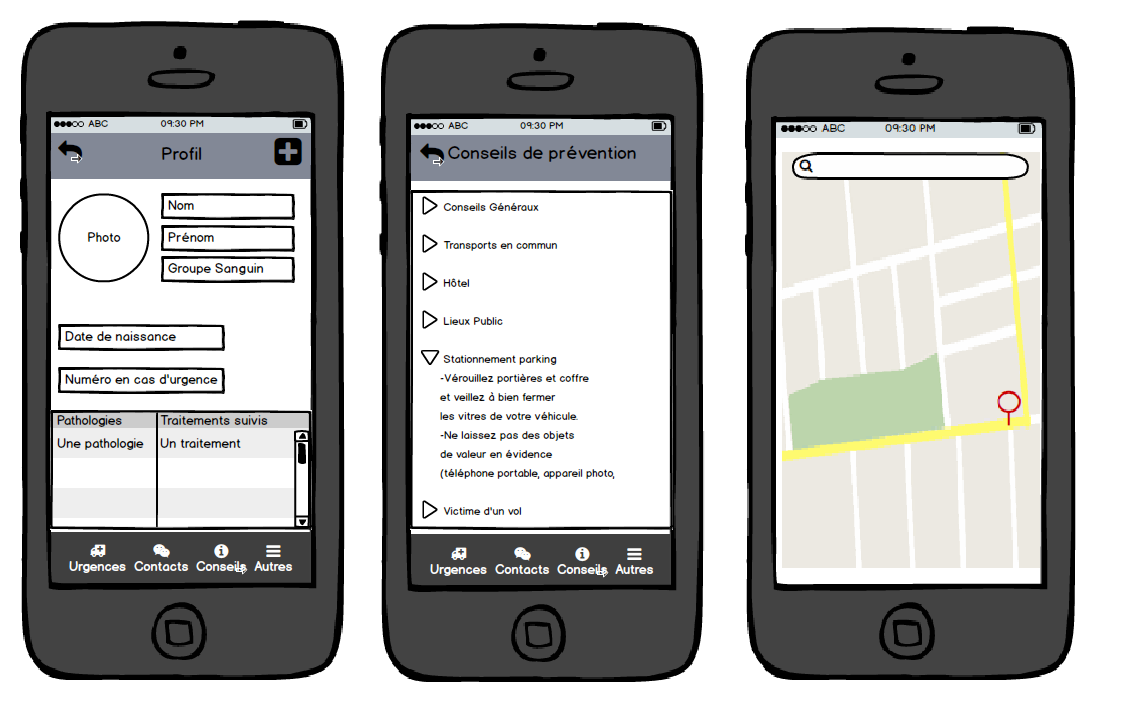
\includegraphics[scale=0.5]{img/maquette2.png}
		\caption{Maquette de l'application : }
		\label{maquette2} 
		
	\end{center}
\end{figure}

\section{Spécifications techniques}
\subsection{Spécifications opérationnelles}

\subsubsection{Caractéristiques techniques}
	L'application sera fonctionnelle sous les systèmes d'exploitation mobile Android en version 4.0 minimum et IOS en version ?. Celle-ci devra être fluide et adaptée à une utilisation tactile. Elle sera proposée à des  utilisateurs ayant des nationalités différentes c'est pourquoi elle devra être lisible et graphique.
	Cette application sera off-line c'est-à-dire sans échange de données direct. Dans le but d'utiliser le module de géolocalisation elle devra faire appel à une application tierce, Google Maps. En outre, elle sera responsive et donc en mesure de s'adapter à différents écrans.

\subsubsection{Permissions}

	L'application nécessitera plusieurs permissions dans l'optique que l'utilisateur puisse profiter pleinement de toutes ses fonctionnalités. Les permissions requises sont les suivantes : 
	\begin{itemize}
		\item \texttt{android.permission.CALL\_PHONE} Autorise l'application à rediriger l'utilisateur sur le composeur téléphonique en lui laissant le choix de confirmer ou non l'appel.
		\item \texttt{android.permission.READ\_EXTERNAL\_STORAGE} Autorise l'application à lire du contenu externe stocké sur le téléphone.
		\item \texttt{android.permission.ACCESS\_COARSE\_LOCATION} Autorise l'application à utiliser les fonctions de géolocalisation approximative.
		\item \texttt{android.permission.ACCESS\_FINE\_LOCATION} Autorise l'application à utiliser les fonctions de géolocalisation de haute précision.
	\end{itemize}
	
\subsection{Outils technologiques}

	\paragraph{}
		Comme nous l'avons expliqué ci-dessus l'application devra être en mesure de fonctionner sous Android et IOS. Cette dernière a déjà été développé en natif sous Android Studio pour le système d'exploitation Android. N'ayant aucune nouvelle de notre client, le choix qui a été fait était de concevoir différente version de l'application afin de pouvoir laisser le client choisir celle qui lui convenait le mieux. Ainsi, nous avons décidé de nous séparer en deux équipes, l'une travaillant sur le développement natif de l'application IOS et l'autre travaillant sur la réalisation d'une application multi plate-forme.
		
	\paragraph{}
		La première équipe composée de Darchen Gautier et Judic Romain a développé une application IOS native à l'aide du langage de programmation Swift et de l'environnement de développement xCode sous macOS. Plus d'informations sur cette partie du projet seront disponibles dans le rapport associé.
		
	\paragraph{}
		En ce qui me concerne, j'ai travaillé sur la réalisation de l'application multi plate-forme. Afin de procéder à cela je me suis tourner vers le développement d'une application hybride, connue pour être bien plus efficace et moins coûteuse en ressource que les applications web cross-platform. Cette application a été réalisée à l'aide du framework \emph{Xamarin} et du langage de programmation \emph{C\#}. Xamarin est disponible gratuitement sous Windows en installant un plugin pour Microsoft Visual Studio ou alors sous MacOS via Xamarin Studio. Ici, l'application a été développée à l'aide de Xamarin Studio. 	 
		   	


\chapter{Conception}
\section{Conception préliminaire}

\subsection{Diagramme de classe}

	Le diagramme présent sur la figure \ref{diagrammeClasse} permet de représenter les différentes activités et classes utilisées dans l'application. 

\begin{sidewaysfigure}
	\includegraphics[scale=0.6]{images/diagrammeClasse.png}
	\caption{Diagramme de classe}
	\label{diagrammeClasse}
\end{sidewaysfigure}

\subsection{Diagramme de navigation}
	
	Le diagramme présent sur la figure \ref{diagrammeNavigation} permet de représenter les transitions entre chaque activité de l'application. 

\begin{figure}[!h]
	\begin{center}
	
	   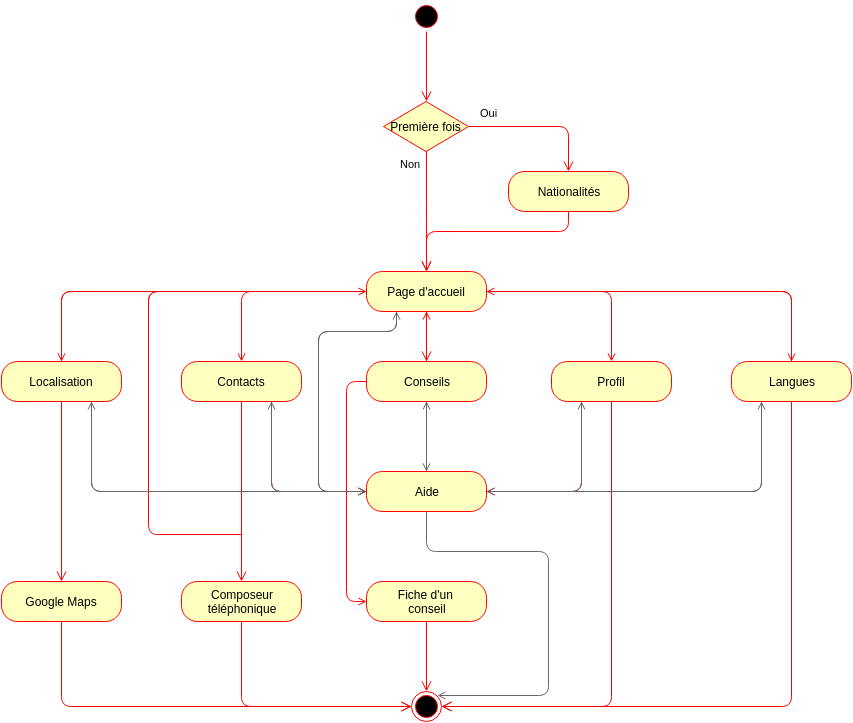
\includegraphics[scale=0.6]{images/navigation.png}
	   \caption{Diagramme de navigation}
	   \label{diagrammeNavigation} 	
	\end{center}
\end{figure}

\section{Conception détaillée}

\subsection{Package JAVA fr.touriste.gendarme.pao.gendarme}
	
\subsubsection{MainActivity}
	
	Cette activité représente l'accueil de l'application. Celle-ci permet à l'utilisateur d'accéder aux différentes fonctionnalités à savoir la localisation de services, la liste de contacts, la liste des conseils, le profil et le choix de la langue. Un raccourci permettant d'appeler les urgences (112) à aussi été placé directement sur l'accueil.
	
	On commence par initialiser la barre de navigation générale de l'application qui sera ensuite disponible à partir de n'importe quelle activité. On construit les différents boutons qui seront présents dans cette dernière à savoir celui permettant d'afficher l'aide ainsi que celui permettant d'ouvrir le menu drawer.
	\\
	
	Si la géolocalisation n'est pas activée l'application demande à l'utilisateur de l'activer dans le but d'accéder à l'apllication et de profiter pleinement de toutes les fonctionnalités disponibles. Ainsi le touriste est automatiquement redirigé dans les options et celui-ci aura le choix d'activer ou non la géolocalisation.
	
\subsubsection{ProfileActivity}
	
	Cette activité permet d'accéder au profil de l'utilisateur. Celui-ci pourra renseigner ses informations personnelles, une photo de profil ainsi que ses remarques médicales.
	\\
	
	On commence par mettre en place les champs texte permettant à l'utilisateur de saisir son nom, son prénom ainsi que son groupe sanguin. On adjoint à ces derniers des valeurs par défaut en fonction de la langue choisie. Ensuite, on met en place le cadre permettant l'affichage de la photo de profil de l'utilisateur. Un clique sur ce cadre le redirige dans la galerie du téléphone afin de sélectionner une image. Celle-ci est automatiquement redimensionnée afin de s'inscrire dans le centre du cadre tout en restant visible. Pour finir, on met en place un tableau permettant au touriste de répertorier les différentes remarques médicales le concernant.
	\\
	
	Dans le but de modifier les informations présentes sur le profil, un bouton \emph{Modification} à été implémenter et à été placé dans la barre de navigation située en haut de l'activité.
	\\
	
	Enfin, l'ensemble des informations entrées par l'utilisateur est sauvegardé en utilisant les préférences Android. De plus, une sécurité à été mise en place pour sauvegarder dans le cas où l'utilisateur modifie ses informations et quitte brusquement l'activité sans passer par le bouton de \emph{Modification}.
	\\
	
	Cette activité est directement accessible depuis la page d'accueil de l'application.

\subsubsection{AdviceActivity}
	Cette activité permet d'afficher une liste de conseils proposés à l'utilisateur. Elle regroupe un ensemble de conduite à tenir en fonction de différentes situations dans lesquelles un touriste étranger pourrait se trouver.
	\\
		
	La liste des conseils présentée dans cette activité est construite de manière dynamique. Le label de chacun des items de la liste doit être consigné dans le fichier XML \emph{strings.xml}. Ensuite, un premier tableau contenant l'ensemble des noms de fichiers HTML représentant les fiches de conseils est construit. Celui récupère l'ensemble des fichiers HTML situés dans le dossier \emph{assets/"langue"/advices} et qui suivent la convention de nomage suivante : \emph{advice\_numero\_ISOLANGUE}. Un second tableau contenant le nom de l'ensemble des images représentant les conseils est construit. Celui-ci récupère l'ensemble des images situés dans le dossier \emph{drawable} et qui suivent la convention de nomage suivante : \emph{image\_advice\_numero}.
	\\
	
	Une fois ces différents tableaux créés, on construit un \texttt{ArrayAdapter} permettant de lier un label avec son image correspondante et de stocker cela dans une \texttt{ListView}. Cette liste est ensuite afficher à l'utilisateur qui n'aura plus qu'à cliquer sur l'item de son choix pour afficher le descriptif du conseil. Pour cela un \emph{listener} est mis en place dans le but de d'appeler l'activité \emph{ReaderActivity} qui sera en charge de d'afficher le contenu du fichier HTML correspondant au conseil.
	\\
	
	Cette activité est directement accessible depuis la page d'accueil de l'application.
		
\subsubsection{ContactActivity}

	Cette activité permet d'afficher une liste contenant l'ensemble des contacts et services pouvant être utile à l'utilisateur. Il s'agit principalement de numéros d'urgence comme les pompiers ou la gendarmerie.
	\\

	Au sein de cette activité on créé un bouton pour chacun des contacts qui sera présent. Ensuite, on leur associe un listener qui permet de rediriger l'utilisateur sur son composeur téléphonique avec le numéro adéquat pré-écrit. Celui-ci aura toujours le choix de confirmer ou non l'appel téléphonique.
	\\
	
	Dans le but de faire appel au composeur téléphonique, cette activité nécessite la permission\\ \emph{android.permission.CALL\_PHONE}. 
	\\
	
	Cette activité est directement accessible depuis la page d'accueil de l'application.

\subsubsection{LanguageActivity}
	
	Cette activité permet d'afficher une liste de nationalités permettant à l'utilisateur de changer la langue de l'application.
	\\
	
	L'ensemble des langues disponibles est consigné dans le fichier XML \emph{strings.xml} dans le tableau \emph{nationalityList} en suivant la convention de nommage suivante : \emph{isolangue:langue}. La liste est ensuite construite en récupérant automatiquement les strings présentes dans le tableau mentionné précédemment. La partie "langue" correspond au label qui sera affiché dans la liste, il est purement décoratif. La partie "isolangue" correspond au code iso de la langue qui permettra à l'application de récupérer automatiquement les fichiers de langue adéquats. Ces fichiers sont stockés dans le dossier \emph{res/values-isolangue}. En outre, cette fonction permet de sauvegarder la langue choisi par l'utilisateur en stockant son choix dans ses préférences.
	\\
	
	Cette activité est accessible depuis le menu \texttt{drawer} (menu déployé en glissant depuis la gauche de l'écran) situé sur l'accueil de l'application.

\subsubsection{LanguageFirstTime}

	Cette activité permet de récupérer la langue sauvegardée dans les préférences de l'utilisateur. Si cette dernière est nulle c'est que l'utilisateur accède pour la première fois à l'application, c'est pourquoi il sera redirigé sur la page permettant le choix d'une langue. Dans le cas contraire il sera envoyé sur la page d'accueil.

\subsubsection{LocalisationActivity}
	
	Cette activité permet d'afficher une liste de services à l'utilisateur et de rediriger ce dernier sur l'application GoogleMaps dans l'optique de localiser le service et de proposer un itinéraire vers ce dernier.
	\\
	
	Le traitement du clic est le même pour chaque option. La seule chose qui va changer dans la redirection est la requête vers GoogleMaps. Si la personne clique sur hôpital alors on choisi cette option là. Voici un exemple de requête : "\texttt{geo:0,0?q=Hôtpital}"
	\\
	
	Cette activité est directement accessible depuis la page d'accueil de l'application.

\subsubsection{HelpActivity}

	Cette activité a pour objectif de fournir une aide d'utilisation de l'application à l'utilisateur. Elle affiche simplement un descriptif permettant d'expliquer comment utiliser chacune des activités présentes au sein de l'application. Cette dernière est accessible depuis la barre de navigation générale de l'application.

\subsubsection{readerActivity}
	
	Cette activité permet d'afficher le contenu d'un fichier HTML contenant les conseils situationnels fournis par la gendarmerie.
	\\
	
	L'outil utilisé est un \texttt{WebView}. Cet outil permet d'afficher une page HTML. On peut y ajouter des options tel que le zoom, activer le JavaScript de la page HTML. On récupère l'item qui a été sélectionné lors de l'appel par l'activité des conseils, on récupère le fichier voulu dans le dossier "Assets" avec la nationalité correspondante. 
	
	
\subsection{Package JAVA fr.touriste.gendarme.pao.gendarme.tools}

\subsubsection{CircularImageview}
	
	Cette classe permet de créer une \texttt{imageView} de forme circulaire avec un bord de couleur et d'épaisseur à définir. Il s'agit du cadre permettant d'accueillir la photo de profil de l'utilisateur. 

\subsubsection{CustomListAdapter}
	
	Il s'agit d'un \texttt{Adapter} permettant d'associer un champs texte et une image afin de d'intégrer ces derniers dans une listView. il s'agit de l'\texttt{Adapter} utilisé dans le but de construire la liste des conseils situationnels.
	
\subsubsection{DataArrayAdapter}

	Cette classe représente un \texttt{Adapter} permettant de construire un tableau et gérer la sauvegardes et les préférences de l'utilisateur vis à vis des informations contenues dans le tableau. Il s'agit de l'adapter utilisé pour construire la liste des remarques médicales dans le profil.
	
	
\subsection{Dossier Assets}
	
	Ce dossier va contenir l'ensemble des données brutes de l'application. Dans notre cas, on y retrouve les documents des conseils au format HTML, mais on peut également y ajouter des fichiers texte, musique et vidéo. Il est composé de 8 dossiers correspondants aux différentes nationalités disponibles de l'application. Ces dossiers permettent de rendre dynamique l'application, en ajoutant un simple fichier avec le bon format ainsi qu'une photo, on ajoute un nouveau conseil dans notre onglet "Conseils". 
	
\subsection{Dossier res}
	
	On y retrouve l'ensemble des ressources qui compose l'application. On identifie différents dossiers :\\
	\begin{itemize}
		\item \textit{anim} : Dossier contenant des fichiers de configuration pour les animations.\\
		\item \textit{drawable} : Dans ce dossier, on y trouve l'ensemble des images de l'application. Les autres dossiers tels que "drawable-hdpi" ou "drawable-xxxhdpi" regroupent les images sous d'autres format. le dossier "drawable" étant le dossier par défaut si il n'y a pas le dossier approprié pour tel téléphone.\\
		\item  \textit{layout} : On y retrouve les fichiers XML des activités qui composent notre application. Ces fichiers XML contiennent l'architecture des activités \\
		\item \textit{menu} : Ce dossier est composé de différents fichiers XML qui servent à l'élaboration des menus qui composent notre application, notamment pour accéder au menu des nationalités ou à l'aide.\\
		\item \textit{mipmap} : Dossier contenant l'icône de lancement de l'application.\\
		\item \textit{values} : Ce dossier contient les différentes caractéristiques de l'application en fonction de la langue et de la version du téléphone. Les dossiers "values-v19" et "values-v21" permettent de changer le style de 'application en fonction de la version du téléphone. Les dossiers "values-fr", "values-de" contiennent un fichier "strings.xml" qui contient l'ensemble des chaîne de caractère de notre application dans les langues de la nationalité. Le dossier "values" est un dossier par défaut (langue anglais). Il contient également d'autres fichiers de configuration comme par exemple la couleur globale de l'application, ou encore les dimensions.\\
		\item \textit{AndroidManifest.xml} est le fichier de configuration globale de l'application, il contient les informations systèmes essentielles au bon fonctionnement de celle-ci.\\
	\end{itemize}

\chapter{Conclusion et perspectives}
	Pour conclure, ce projet d’approfondissement et d'ouverture nous a permis d'apprendre à concevoir et développer une application Android. Nous avons découvert, à travers ce projet, de nouvelles technologies et avons pu acquérir de nouvelles expériences en nous initiant à des concepts qui nous étaient jusqu'alors inconnus.
	\\
	
	 Ensuite le développement de cette application nous aura permis de fournir un travail pour un client avec de réelles attentes. Ce client n'étant pas initié au domaine de la programmation, ce projet nous aura permis de nous familiariser avec la création d'un outils simplifié et accessible. De plus, le fait que le client soit la gendarmerie nous a inspiré une certaine motivation supplémentaire.
	 \\
	
	Concernant les perspectives de cette application, un premier point qui pourrait être amélioré concerne la liste des contacts téléphoniques. En effet, il peut être intéressant de rendre la construction de cette liste dynamique à l'image de celle des conseils et mettre en place la possibilité d'ajouter des numéros. Ensuite, un autre point très important concerne la version minimale d'Android avec laquelle l'application est compatible. Par exemple, dans notre cas la barre de navigation générale n'est pas compatible avec la version 2.3 d'Android c'est pourquoi il serait intéressant de trouver une alternative à cette dernière. Enfin, l'application sera testée en situation réelle par le client durant les mois de juin, juillet et août. Celui-ci nous fera part de ses remarques et des différents bugs rencontrés que nous pourrons alors étudier plus en profondeur.

% Bibliographie
%\bibliographystyle{plain}
\printbibliography

% Annexes
%\clearpage
%\appendix
%\chapter{Annexes}
%\input{parties/10-Annexe.tex}


% pageQuatriemeCouverture 
% #1 : Direction
% #2 : telephone
% #3 : e-mail
% #4 : Resume Haut
% #5 : Resume Bas
\pageQuatriemeCouverture{Département ASI}{02 32 95 97 79}{asi@insa-rouen.fr}{}{}

\end{document}
